\newpage
\section{Same Flavor final state}\label{sec:SF}
The analysis for the same-flavor final state $\mathrm{W^+W^-}\to \mu^{\pm}
\mu^{\mp}  2\nu$ and  $\mathrm{W^+W^-}\to e^{\pm} e^{\mp}  2\nu$ is
described here. Also in this case signal and control regions are
defined, but only for the VBF topology is considered. 
\subsection*{Signal region}
Events are requested to pass single or double lepton triggers and all the
physics objects definitions are the same as in the OF analysis.
The final state consists of two well identified electrons or two muons with
$p_T >$ 20 GeV, opposite charge, and large missing transverse energy from the undetected neutrinos.\\
In addition to the backgrounds described for the OF final state, the
background from $\mathrm{DY}\to \mu^{+} \mu^{-}$ and
$\mathrm{DY}\to e^{+} e^{-}$ is very large in this final state,
actually the most important. 
Indeed, due to this very large background, the SF analysis only targets the
VBF topology, where the DY background is suppressed by the tight 
jet requirements. In addition, an invariant mass of the two leptons larger
than 120~\GeV is requested.
The full selection, defined as the ``WW same flavour selection'', is :
\begin{itemize}
\item Two isolated leptons with same flavor and opposite charge ($\mu ^{\pm} \mu^{\mp}$ and $e^{\pm} e^{\mp}$);
\item $p_T$ of the leading and trailing lepton $>$ 20 GeV;
\item Third lepton veto: events are rejected if there is a third lepton with $p_T  >$ 10 GeV;
\item  $m_{\ell \ell} >$ 120 GeV 
\item $p_T^{\ell \ell} >$30 GeV;
\item MET $>$ 50 GeV;
\item $m_T^I >$ 100 GeV;
\item At lest 2 jets non b-tagged (according to CMVA loose WP) with $p_T >$ 30 GeV.
\item $\Delta \eta_{jj} > 3.5$;
\item $m_{jj} >$ 500 GeV;;
\end{itemize}
Similarly to the opposite-flavour analysis, the signal is extracted from a template fit of
the $m_T^I$ distribution.
The $m_T^I$ distributions has the following binning:
\begin{itemize}
\item {\bf VBF}, [100,150,200,250,300,350,400,450,500,600,700,1000];
\end{itemize}
where the first number represents the lower edge of the first bin while the other numbers represent the upper edges. The last bin is an overflow bin. 
The binning has been chosen in order to have at least 10 expected Top-backgrounds events and at least 10  expected  Drell-Yan events in each bin of the template.\\
The distributions in the signal region of the $m_T^I$ variable is shown in  Fig.~\ref{fig:mti_sigOF_Un_log} 
\begin{figure}[htbp]
\centering
\subfigure[ee]{
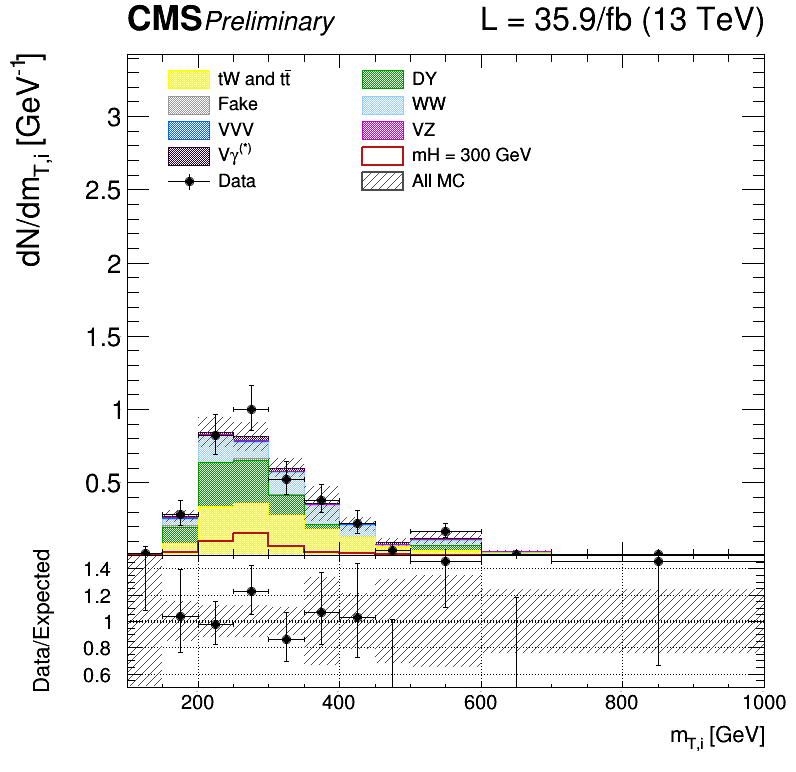
\includegraphics[width=0.45\textwidth]{../AN/Figs/unblinding/plot_SR/plotHWWhighMass_SF_ee_postfit_300/cratio_hwwhm_13TeV_sfVBF_ee_mTi.png}
}
\subfigure[mm]{
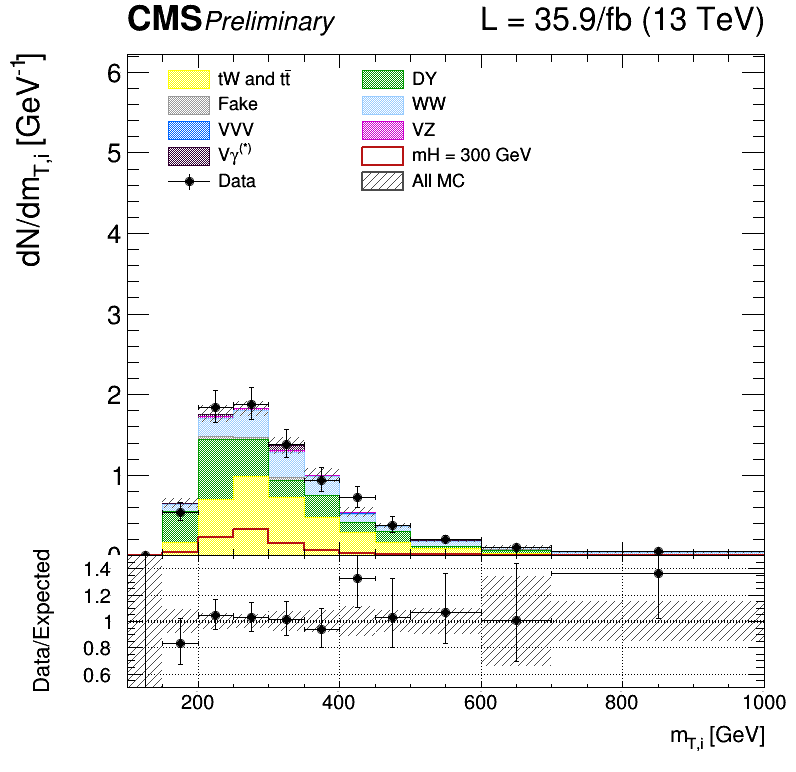
\includegraphics[width=0.45\textwidth]{../AN/Figs/unblinding/plot_SR/plotHWWhighMass_SF_mm_postfit_300/cratio_hwwhm_13TeV_sfVBF_mm_mTi.png}
}
\\
\subfigure[ee]{
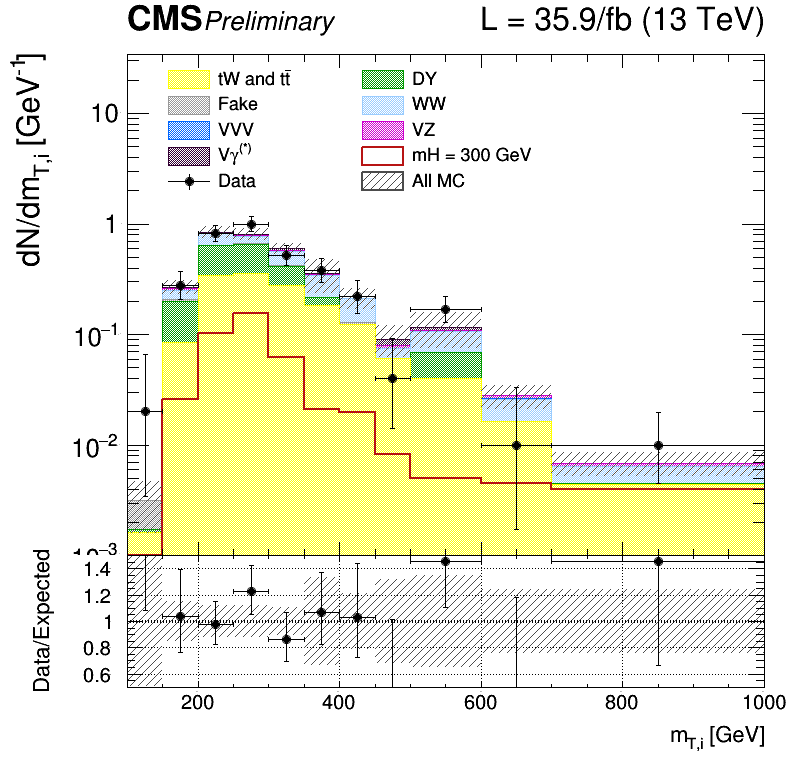
\includegraphics[width=0.45\textwidth]{../AN/Figs/unblinding/plot_SR/plotHWWhighMass_SF_ee_postfit_300/log_cratio_hwwhm_13TeV_sfVBF_ee_mTi.png}
}
\subfigure[mm]{
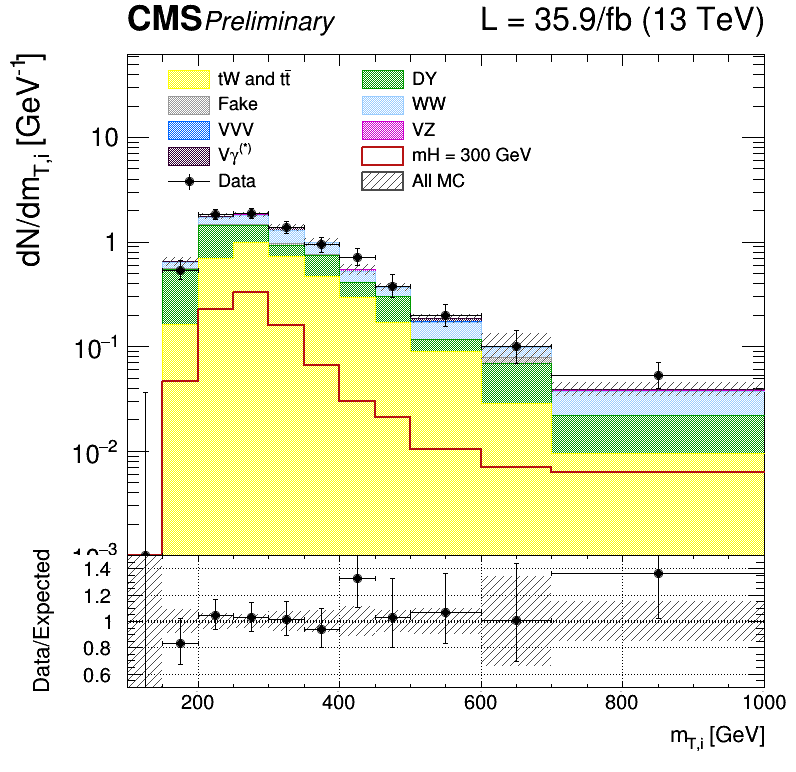
\includegraphics[width=0.45\textwidth]{../AN/Figs/unblinding/plot_SR/plotHWWhighMass_SF_mm_postfit_300/log_cratio_hwwhm_13TeV_sfVBF_mm_mTi.png}
}
\caption{Unblinded distributions  $m_T^I$ in the signal region for $ee$ and $\mu \mu$ categories in linear and log scale. The signal hypothesis corresponds to $m_X $ of 300 GeV.}
    \label{fig:mti_sigOF_Un}
\end{figure}




\newpage

\subsection*{Drell-Yan control region}
The main background for the SF analysis is the DY. 
A control region has been defined, as close as possible to the signal one to
be used for the normalization of the DY background, separately for electrons
and muons.
The control region is defined by the ``WW same flavour selection'', except for the
$m_{\ell \ell}$ requirement which is changed to 70 GeV $ <m_{\ell \ell} <$ 120
GeV to include the Z boson.
The missing transverse energy distribution in the data shows discrepancies with respect to Monte Carlo simulation in ee and $\mu \mu$ DY control regions. A correction is therefore applied by reweighting all the simulated samples with a weight per event which depends on the MET value. 
The weight is evaluated as the ratio between data, once all backgrounds, except the DY, have been subtracted, and the DY itself. This procedure is applied in each bin of the distribution, separately for ee and $\mu \mu$ categories. The weight is assumed to be linear as a function of the MET value.\\
This kind of reweighting allows to correct for shape differences between data and MC, Fig. \ref{fig:dy_met}.
The control plots for several variables in a DY enriched phase space
%for the ee and $\mu \mu$
are shown in Figs.~\ref{fig:mll_sigSF_CR_DY_ee} for
the dielectron case and Figs.~\ref{fig:mll_sigSF_CR_DY_mm} for the dimuon
case. In general there is a good agreement between data and MC.

\newpage

\begin{figure}[htbp]
\centering
\subfigure[ee before the re-weight]{
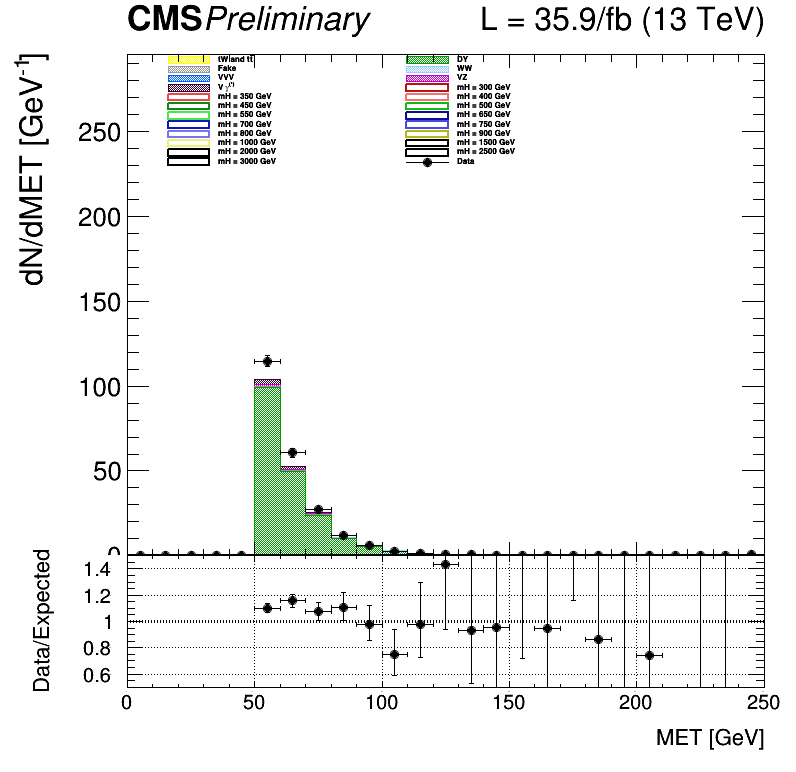
\includegraphics[width=0.45\textwidth]{../AN/Figs/METrw/cratio_hww2l2v_13TeV_dy_e_e_2j_VBF_metPfType1.png}
}
\subfigure[$\mu \mu$  before the re-weight]{
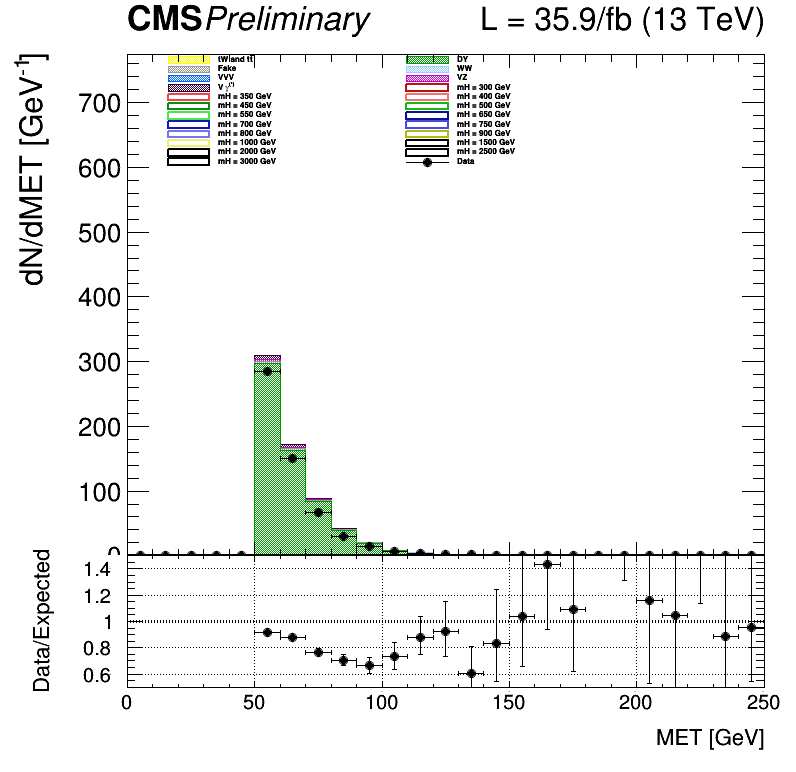
\includegraphics[width=0.45\textwidth]{../AN/Figs/METrw/cratio_hww2l2v_13TeV_dy_mu_mu_2j_VBF_metPfType1.png}
}                                              

\subfigure[ee  after the re-weight]{
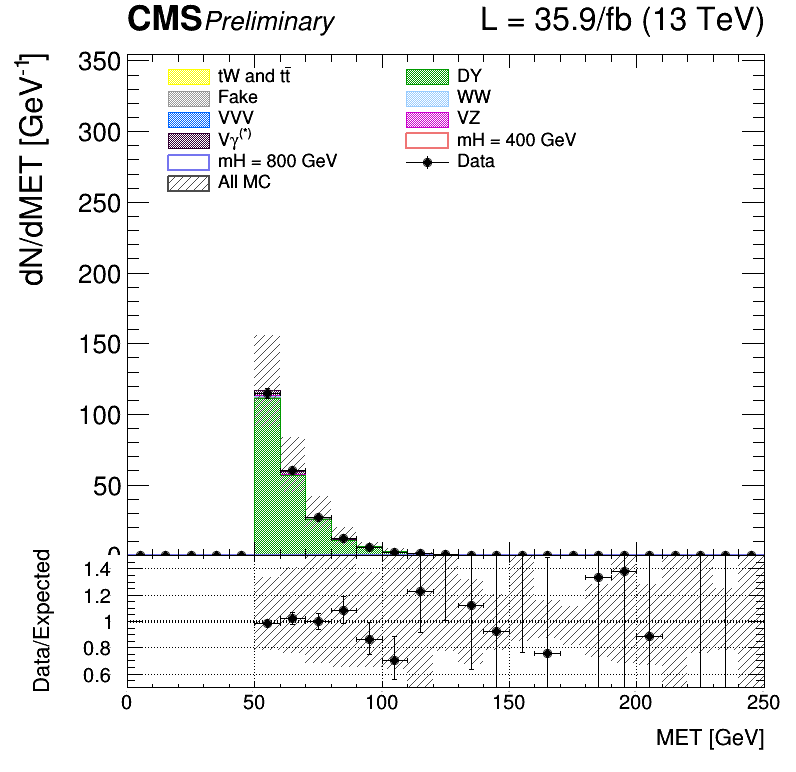
\includegraphics[width=0.45\textwidth]{../AN/Figs/SF_CR_Blind/cratio_hww2l2v_13TeV_dy_e_e_2j_VBF_metPfType1.png}
}
\subfigure[$\mu \mu$  after the re-weight]{
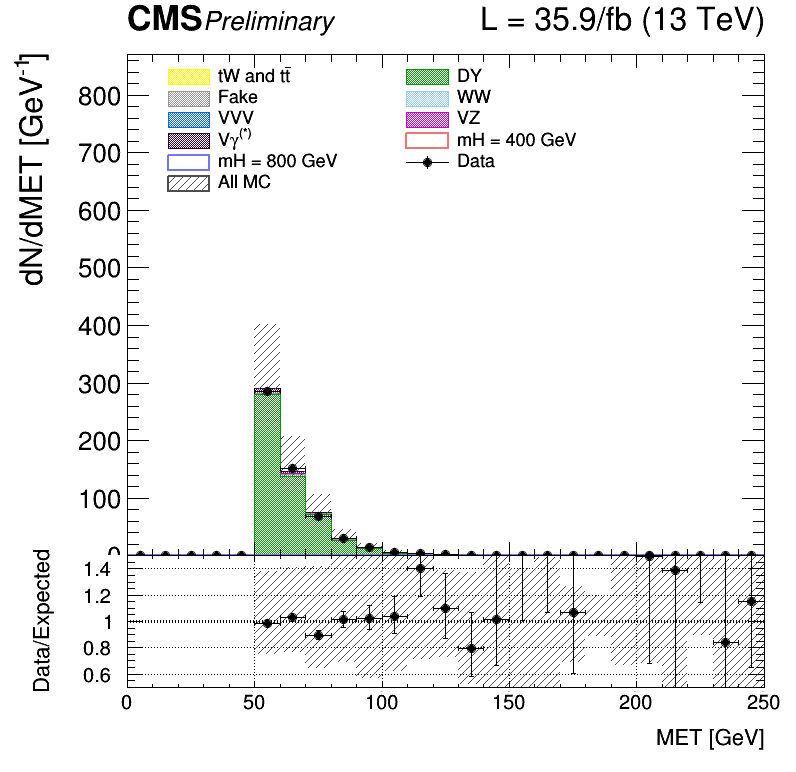
\includegraphics[width=0.45\textwidth]{../AN/Figs/SF_CR_Blind/cratio_hww2l2v_13TeV_dy_mu_mu_2j_VBF_metPfType1.png}
}                   

\caption{MET control plots for Drell-Yan in the ee categories \textit{a} and $\mu \mu$ \textit{b} categories before the reweighting. In \textit{c} and  \textit{d} the same 
distribution after the correction.}
    \label{fig:dy_met}                                             

\end{figure}




\newpage

\begin{figure}[htbp]
\centering
\subfigure[$m_T^I$]{
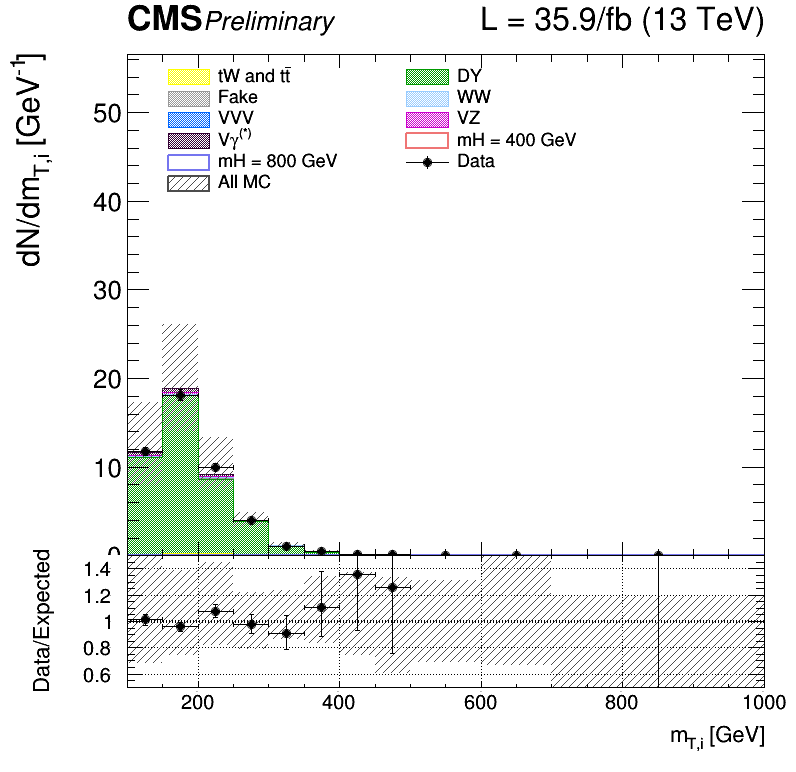
\includegraphics[width=0.45\textwidth]{../AN/Figs/SF_CR_Blind/cratio_hww2l2v_13TeV_dy_e_e_2j_VBF_mTi.png}
}
\subfigure[$m_T^H$]{
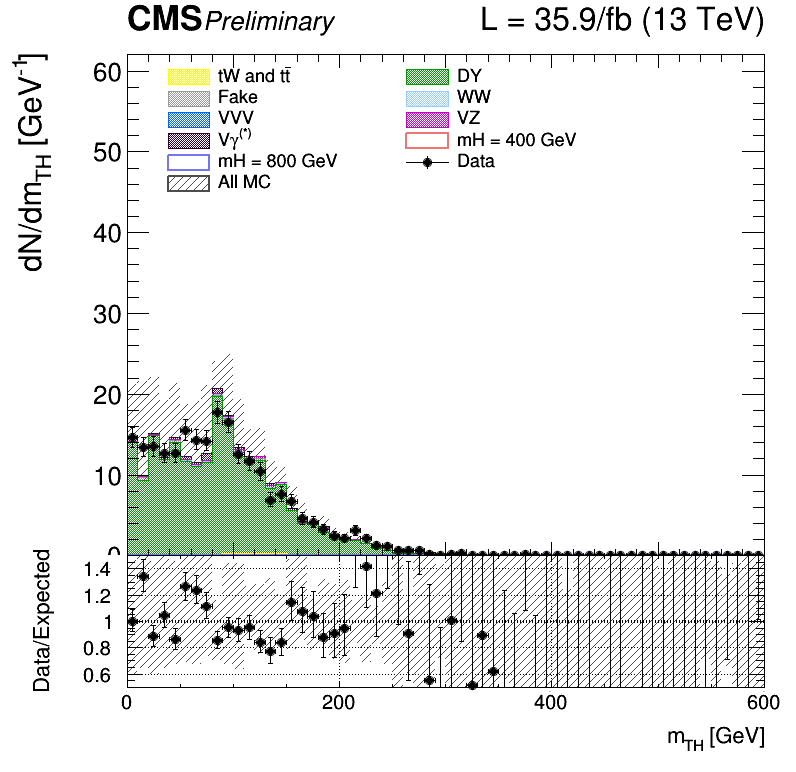
\includegraphics[width=0.45\textwidth]{../AN/Figs/SF_CR_Blind/cratio_hww2l2v_13TeV_dy_e_e_2j_VBF_mth.png}
}                                              
\\                                             
\subfigure[$m_{jj}$]{                             
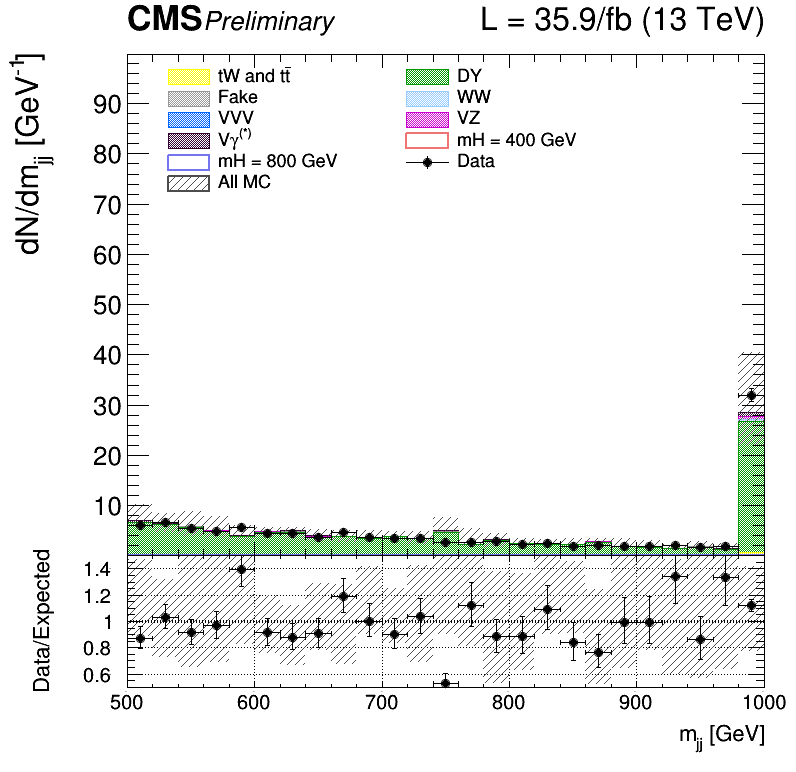
\includegraphics[width=0.45\textwidth]{../AN/Figs/SF_CR_Blind/cratio_hww2l2v_13TeV_dy_e_e_2j_VBF_mjj_DY.png}
}                                              
\subfigure[$m_{\ell \ell}$]{                               
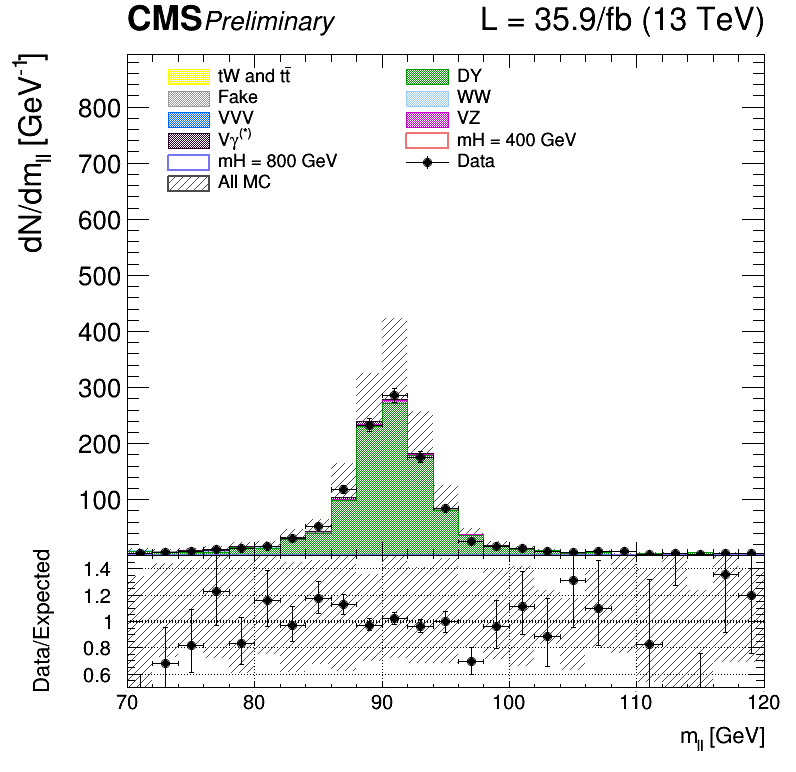
\includegraphics[width=0.45\textwidth]{../AN/Figs/SF_CR_Blind/cratio_hww2l2v_13TeV_dy_e_e_2j_VBF_mll.png}
}\\

\subfigure[$p_T$ leading lepton]{                             
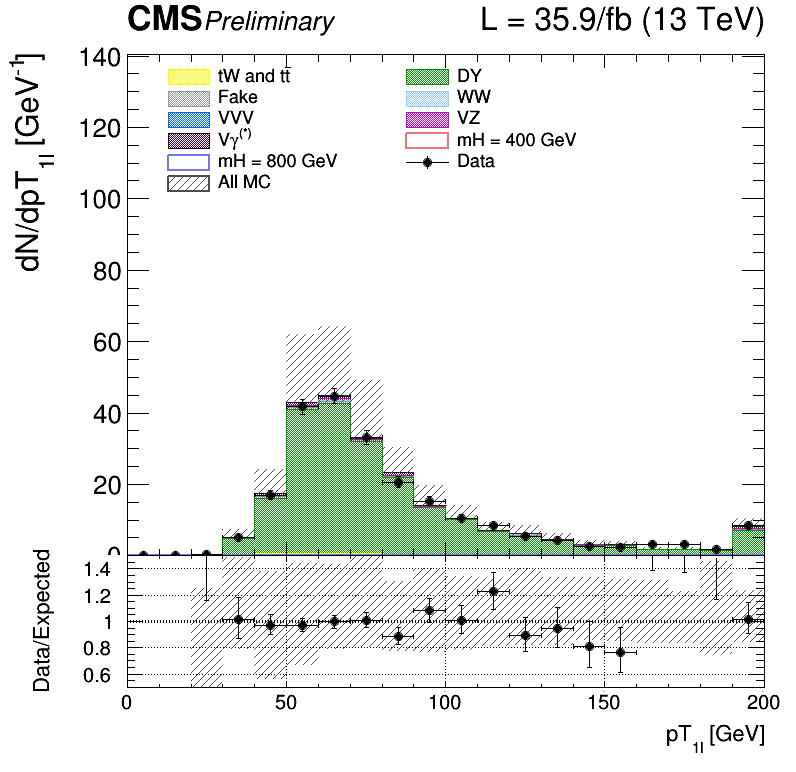
\includegraphics[width=0.45\textwidth]{../AN/Figs/SF_CR_Blind/cratio_hww2l2v_13TeV_dy_e_e_2j_VBF_std_vector_lepton_pt[0].png}
}                                              
\subfigure[$p_T^{\ell \ell}$]{                               
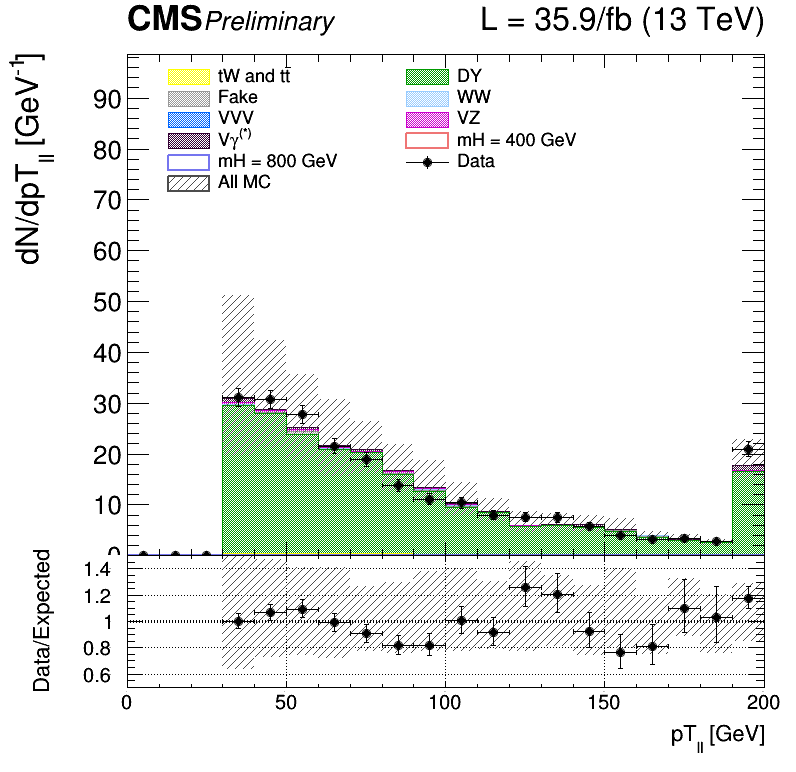
\includegraphics[width=0.45\textwidth]{../AN/Figs/SF_CR_Blind/cratio_hww2l2v_13TeV_dy_e_e_2j_VBF_ptll.png}
}\\

\caption{Control plots for several variables in a Drell-Yan enriched phase space for ee.}
    \label{fig:mll_sig}
\end{figure}

\newpage

\begin{figure}[htbp]
\centering
\subfigure[$m_T^I$]{
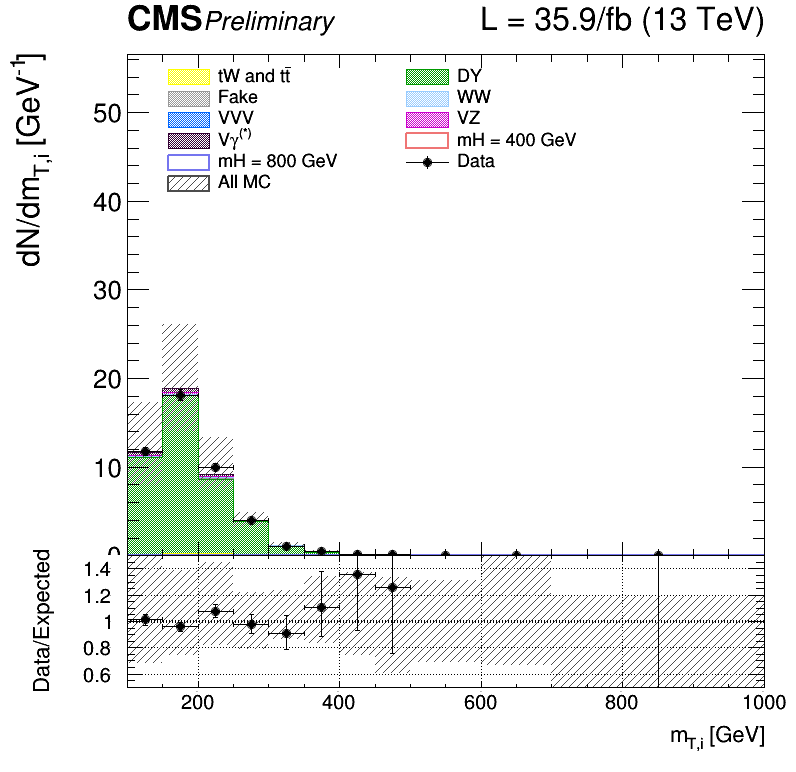
\includegraphics[width=0.45\textwidth]{../AN/Figs/SF_CR_Blind/cratio_hww2l2v_13TeV_dy_e_e_2j_VBF_mTi.png}
}
\subfigure[$m_T^H$]{
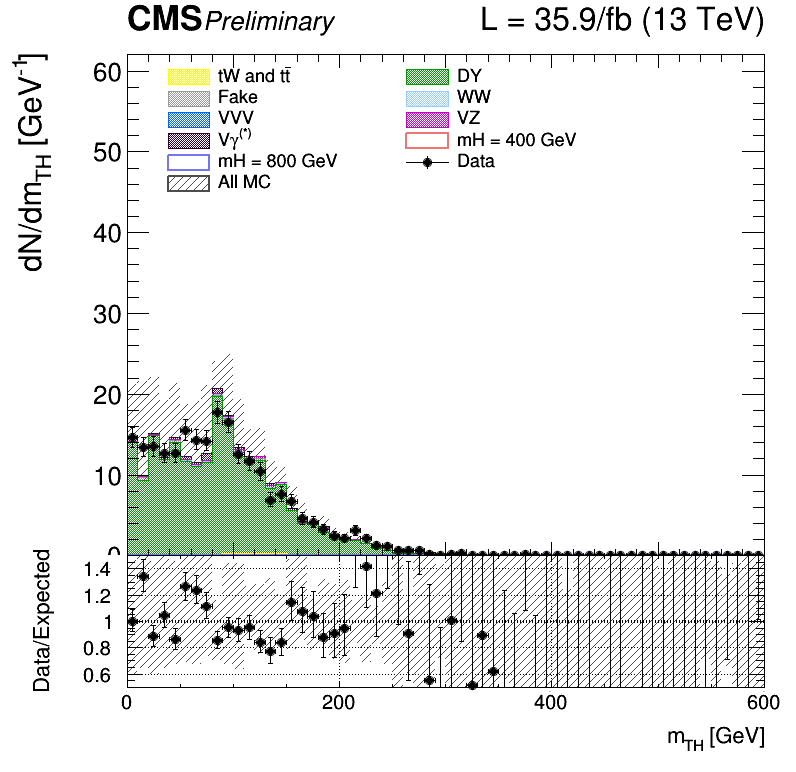
\includegraphics[width=0.45\textwidth]{../AN/Figs/SF_CR_Blind/cratio_hww2l2v_13TeV_dy_e_e_2j_VBF_mth.png}
}                                              
\\                                             
\subfigure[$m_{jj}$]{                             
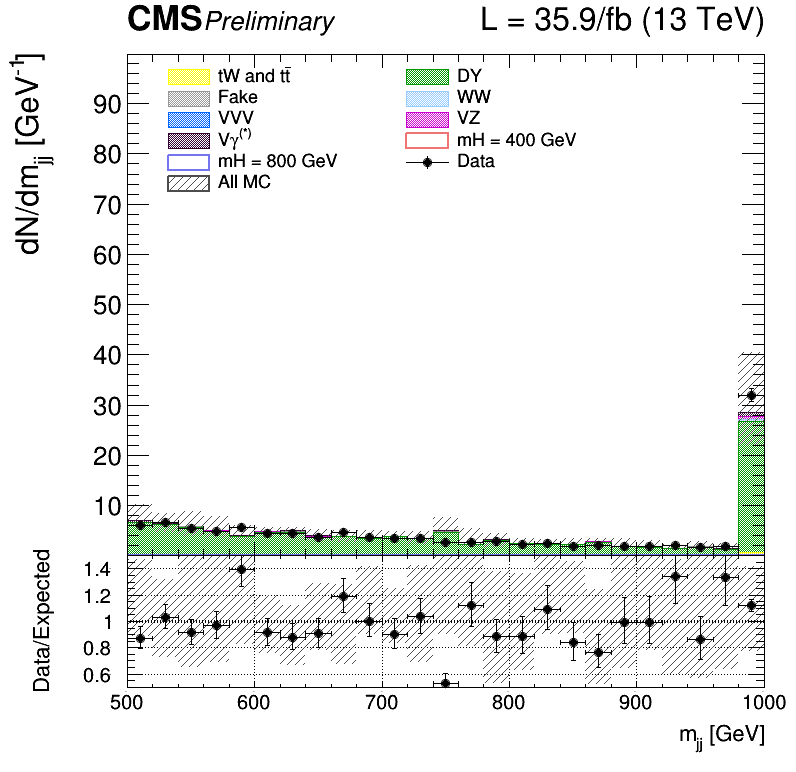
\includegraphics[width=0.45\textwidth]{../AN/Figs/SF_CR_Blind/cratio_hww2l2v_13TeV_dy_e_e_2j_VBF_mjj_DY.png}
}                                              
\subfigure[$m_{\ell \ell}$]{                               
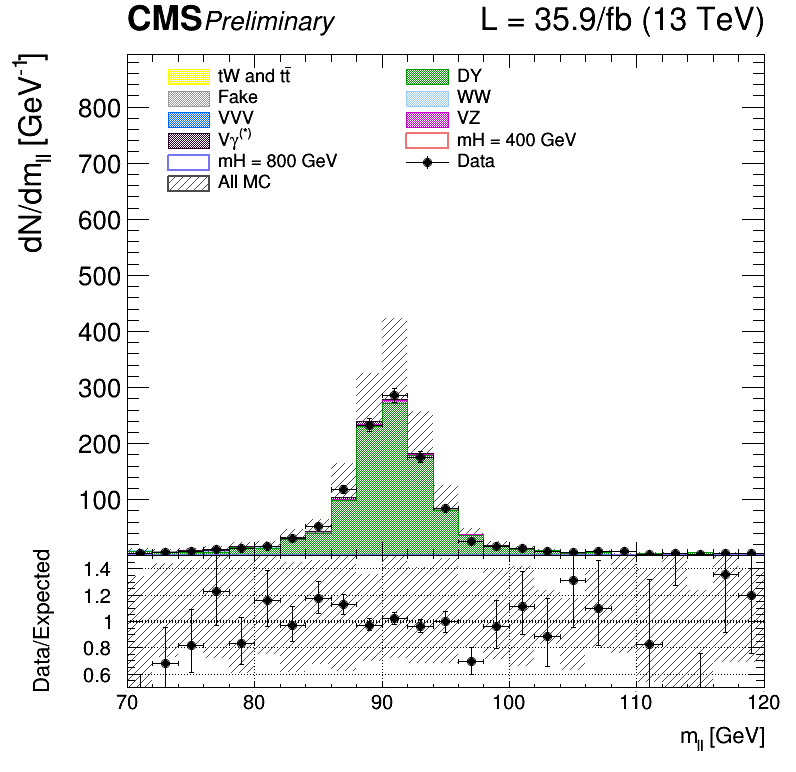
\includegraphics[width=0.45\textwidth]{../AN/Figs/SF_CR_Blind/cratio_hww2l2v_13TeV_dy_e_e_2j_VBF_mll.png}
}\\

\subfigure[$p_T$ leading lepton]{                             
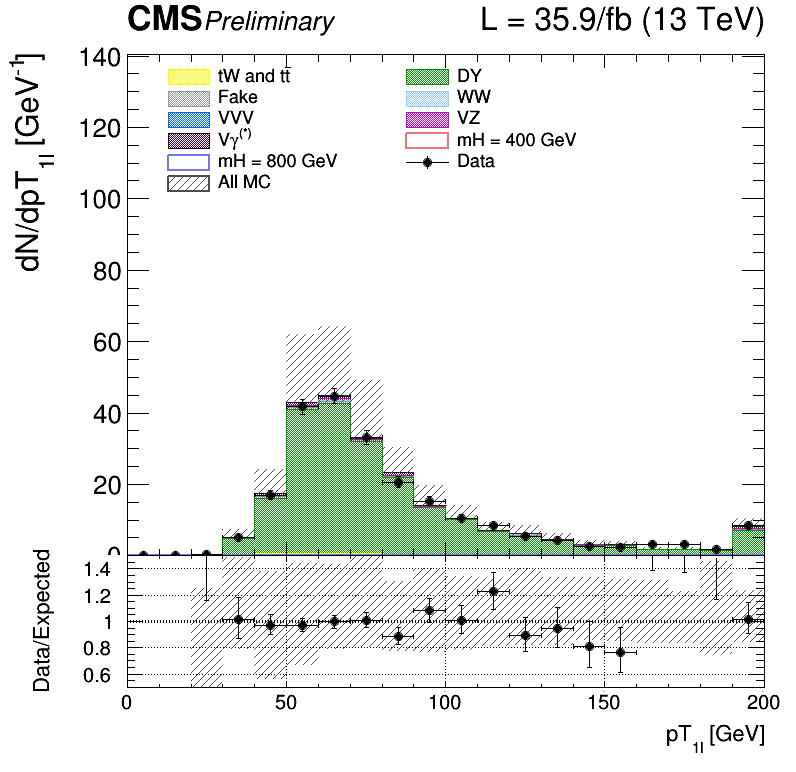
\includegraphics[width=0.45\textwidth]{../AN/Figs/SF_CR_Blind/cratio_hww2l2v_13TeV_dy_e_e_2j_VBF_std_vector_lepton_pt[0].png}
}                                              
\subfigure[$p_T^{\ell \ell}$]{                               
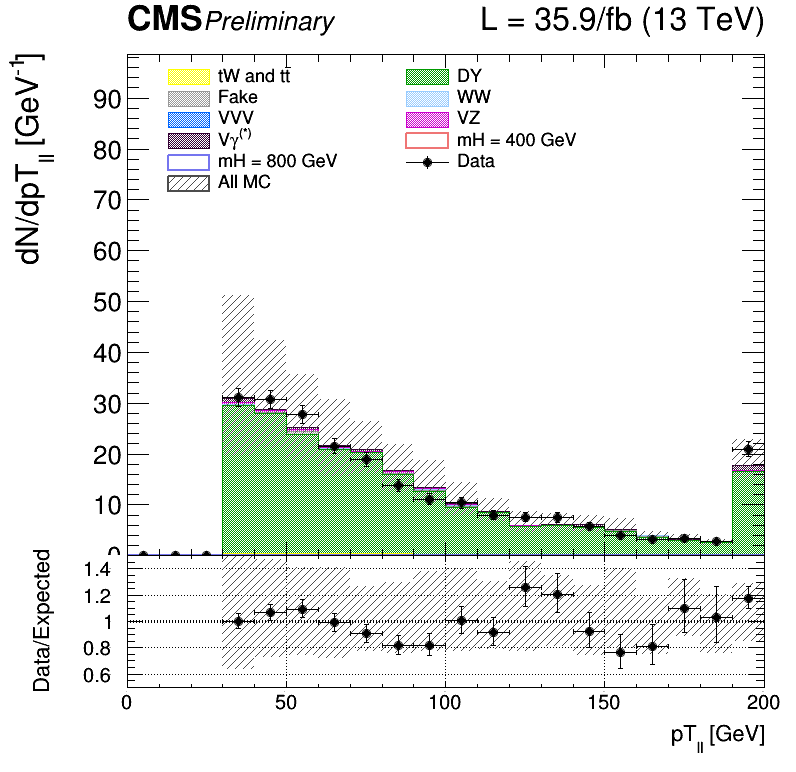
\includegraphics[width=0.45\textwidth]{../AN/Figs/SF_CR_Blind/cratio_hww2l2v_13TeV_dy_e_e_2j_VBF_ptll.png}
}\\

\caption{Control plots for several variables in a Drell-Yan enriched phase space for ee.}
    \label{fig:mll_sigSF_CR_DY_ee}
\end{figure}


\newpage

\begin{figure}[h]
\centering
\subfigure[$m_T^I$]{
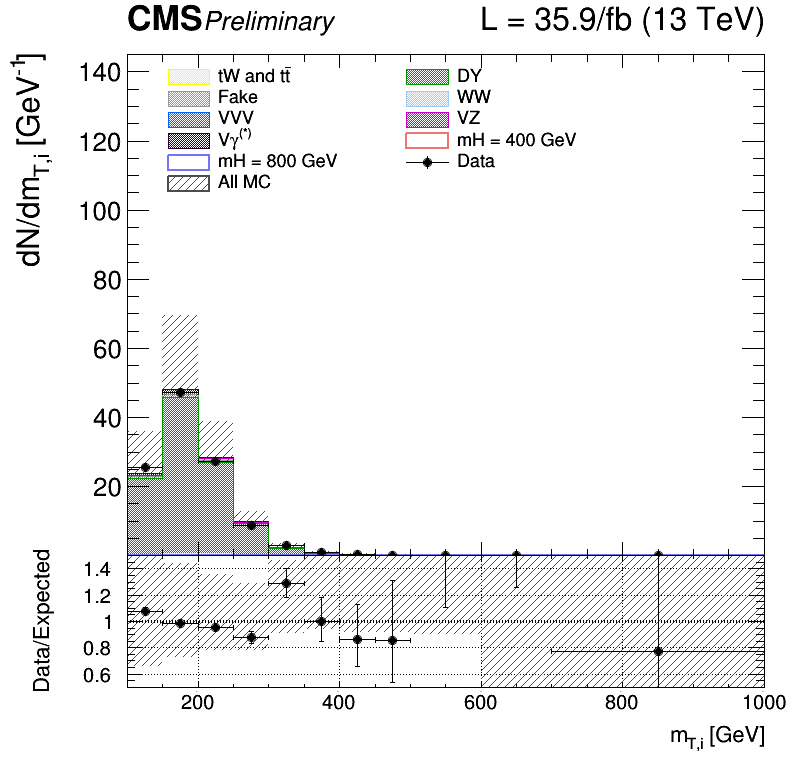
\includegraphics[width=0.45\textwidth]{../AN/Figs/SF_CR_Blind/cratio_hww2l2v_13TeV_dy_mu_mu_2j_VBF_mTi.png}
}
\subfigure[$m_T^H$]{
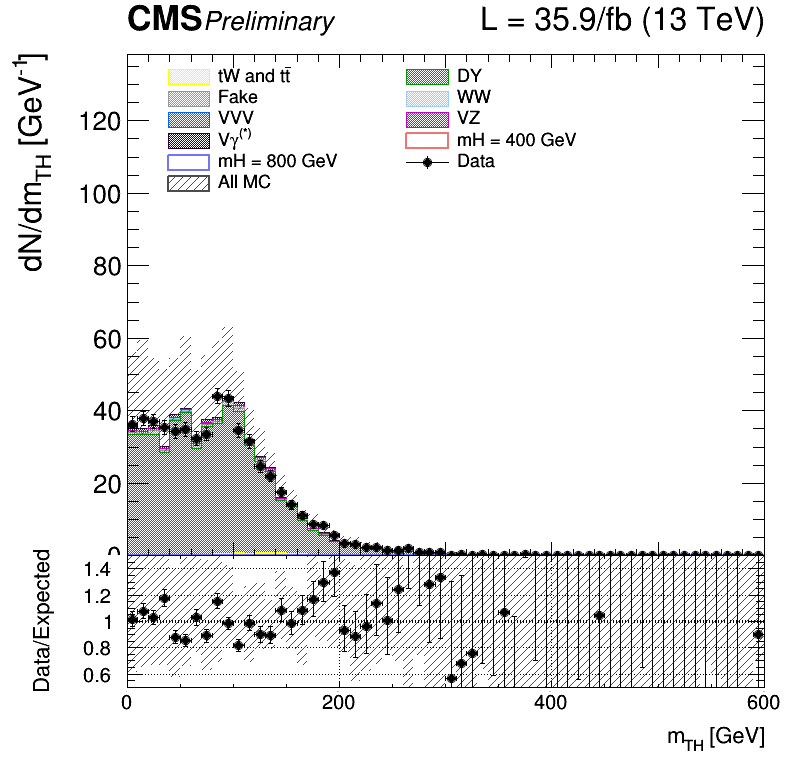
\includegraphics[width=0.45\textwidth]{../AN/Figs/SF_CR_Blind/cratio_hww2l2v_13TeV_dy_mu_mu_2j_VBF_mth.png}
}                                              
\\                                             
\subfigure[$m_{jj}$]{                             
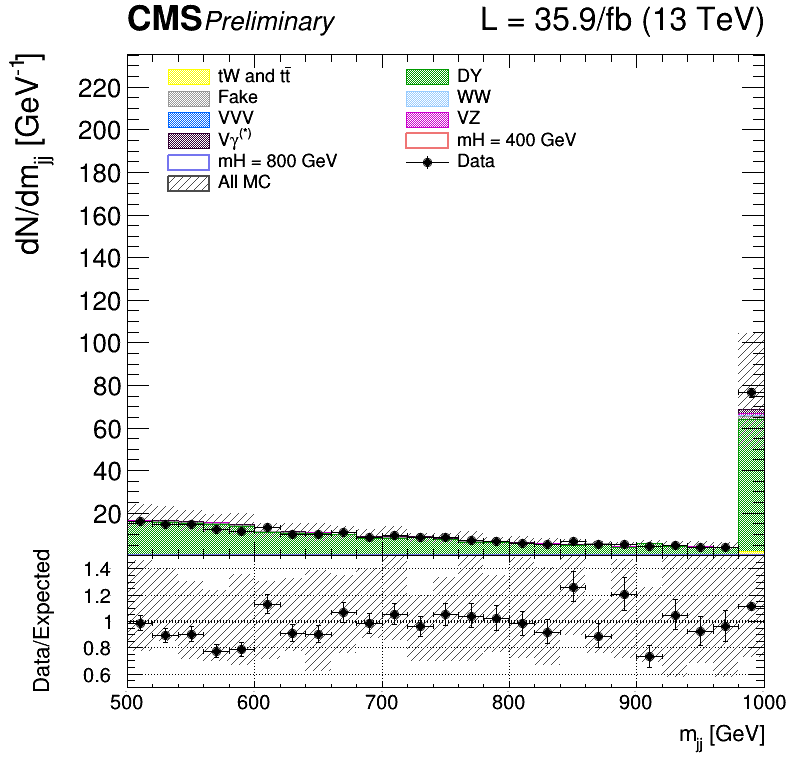
\includegraphics[width=0.45\textwidth]{../AN/Figs/SF_CR_Blind/cratio_hww2l2v_13TeV_dy_mu_mu_2j_VBF_mjj_DY.png}
}                                              
\subfigure[$m_{\ell \ell}$]{                               
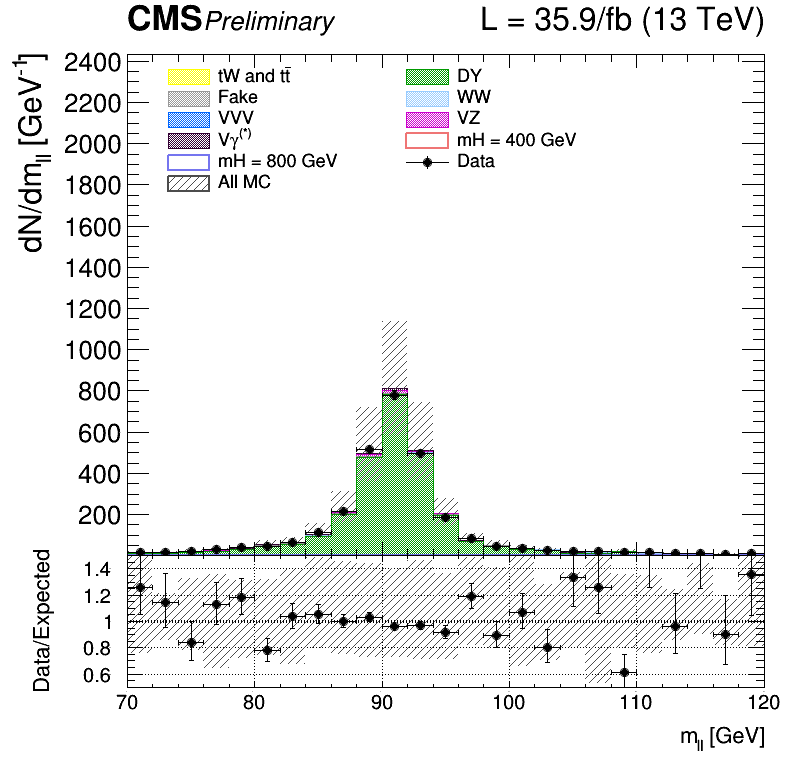
\includegraphics[width=0.45\textwidth]{../AN/Figs/SF_CR_Blind/cratio_hww2l2v_13TeV_dy_mu_mu_2j_VBF_mll.png}
}\\

\subfigure[$p_T$ leading lepton]{                             
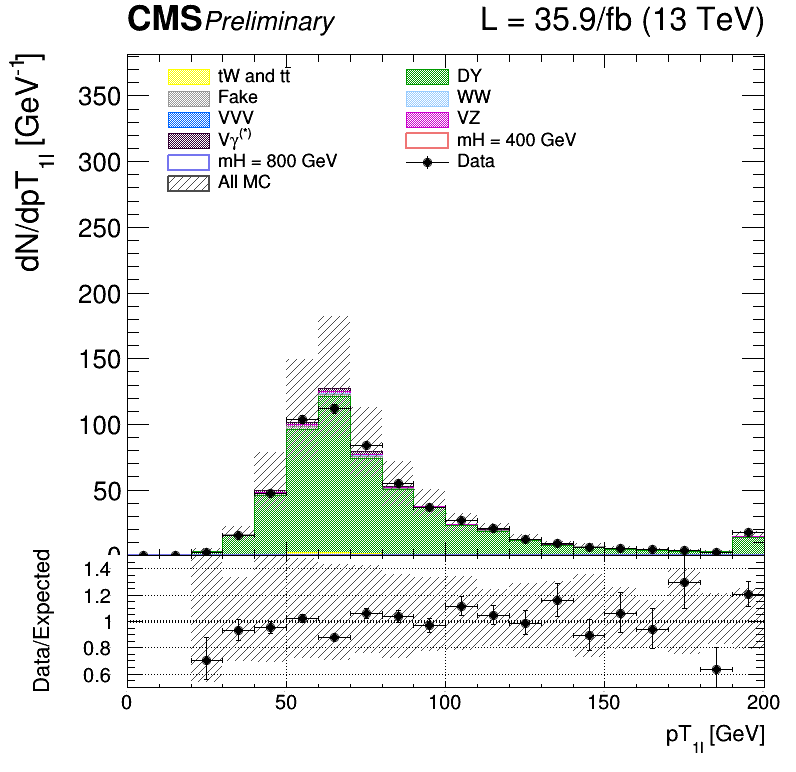
\includegraphics[width=0.45\textwidth]{../AN/Figs/SF_CR_Blind/cratio_hww2l2v_13TeV_dy_mu_mu_2j_VBF_std_vector_lepton_pt[0].png}
}                                              
\subfigure[$p_T^{\ell \ell}$]{                               
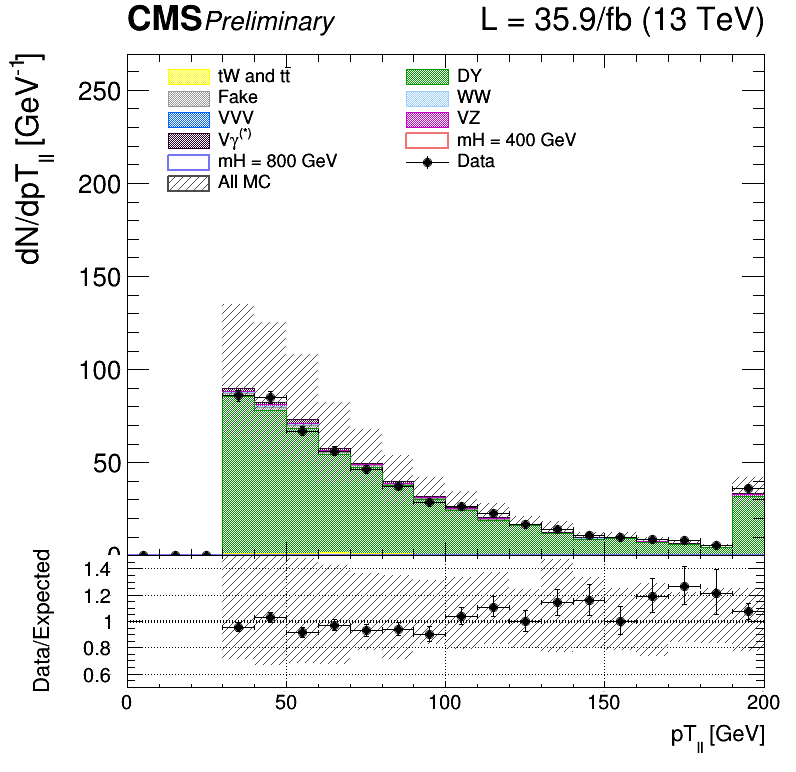
\includegraphics[width=0.45\textwidth]{../AN/Figs/SF_CR_Blind/cratio_hww2l2v_13TeV_dy_mu_mu_2j_VBF_ptll.png}
}\\

\caption{Control plots for several variables in a Drell-Yan enriched phase space for $\mu \mu$.}
    \label{fig:mll_sigSF_CR_DY_mm}
\end{figure}

\newpage
\clearpage
\subsection*{Top control region}
A top-enriched control region is defined to normalize the top backgrounds,
separately for electrons and muons.
The ``WW SF selection'' is required with the inversion of the b-tagging
requirement, i.e. the two jets are both requested to be b-tagged according to
CMVA loose WP.
The control plots for several variables in a top enriched phase space for events are shown in
the Figs.~\ref{fig:mll_sigSF_CR_top_ee} for the dielectron case and
\ref{fig:mll_sigSF_CR_top_mm} for the dimuon case. Good agreement is observed
between data and MC.


\begin{figure}[htbp]
\centering
\subfigure[$m_T^I$]{
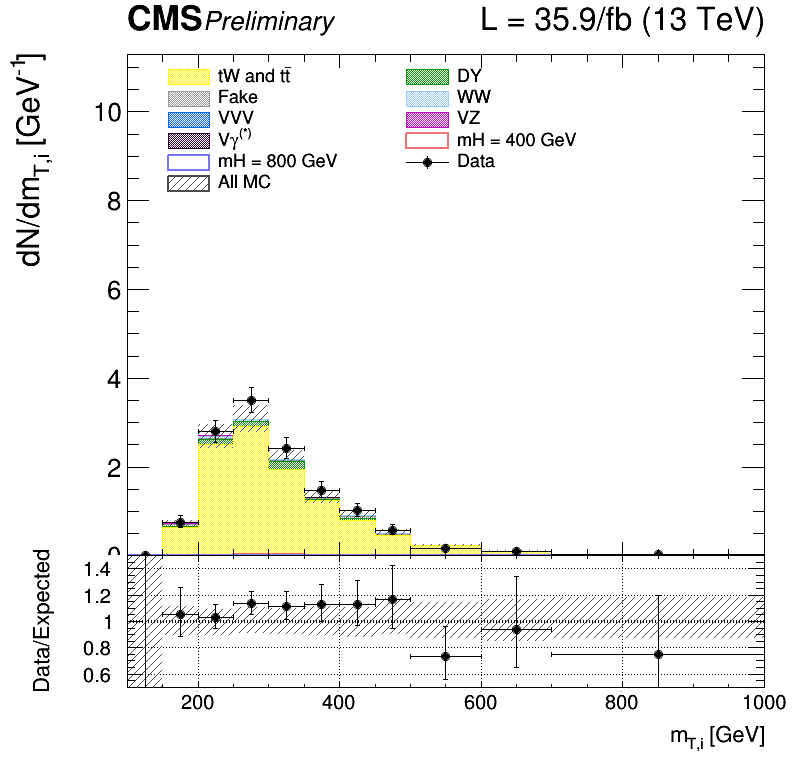
\includegraphics[width=0.45\textwidth]{../AN/Figs/SF_CR_Blind/cratio_hww2l2v_13TeV_top_e_e_2j_VBF_mTi.png}
}
\subfigure[$m_T^H$]{
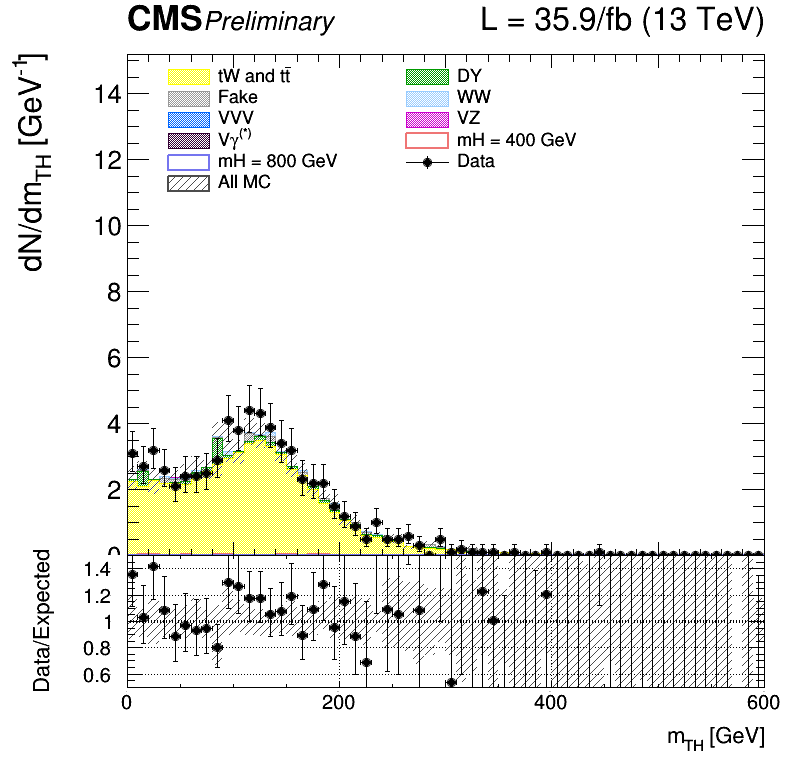
\includegraphics[width=0.45\textwidth]{../AN/Figs/SF_CR_Blind/cratio_hww2l2v_13TeV_top_e_e_2j_VBF_mth.png}
}                                              
\\                                             
\subfigure[$m_{jj}$]{                             
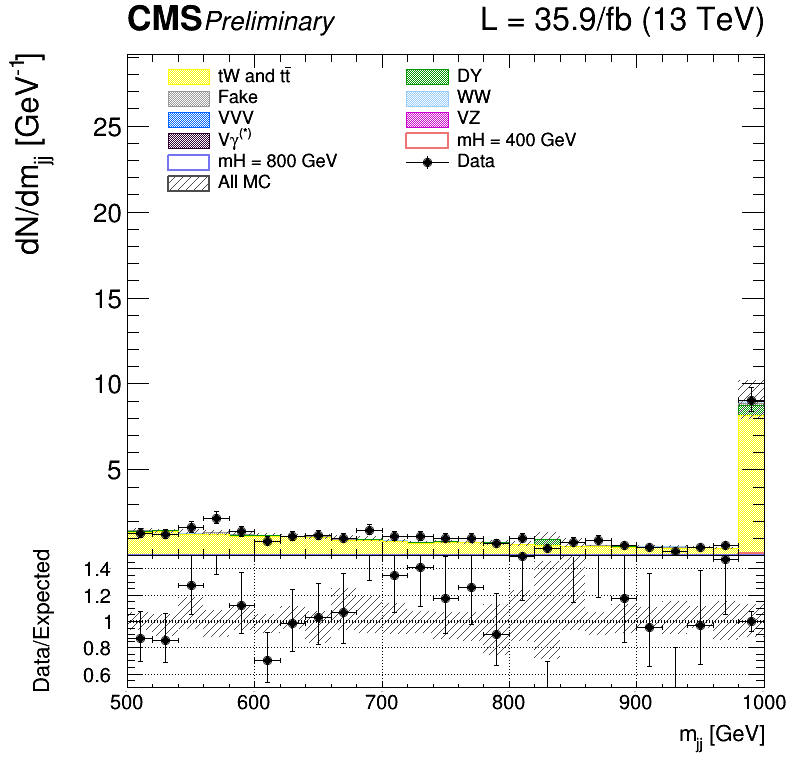
\includegraphics[width=0.45\textwidth]{../AN/Figs/SF_CR_Blind/cratio_hww2l2v_13TeV_top_e_e_2j_VBF_mjj_DY.png}
}                                              
\subfigure[$m_{\ell \ell}$]{                               
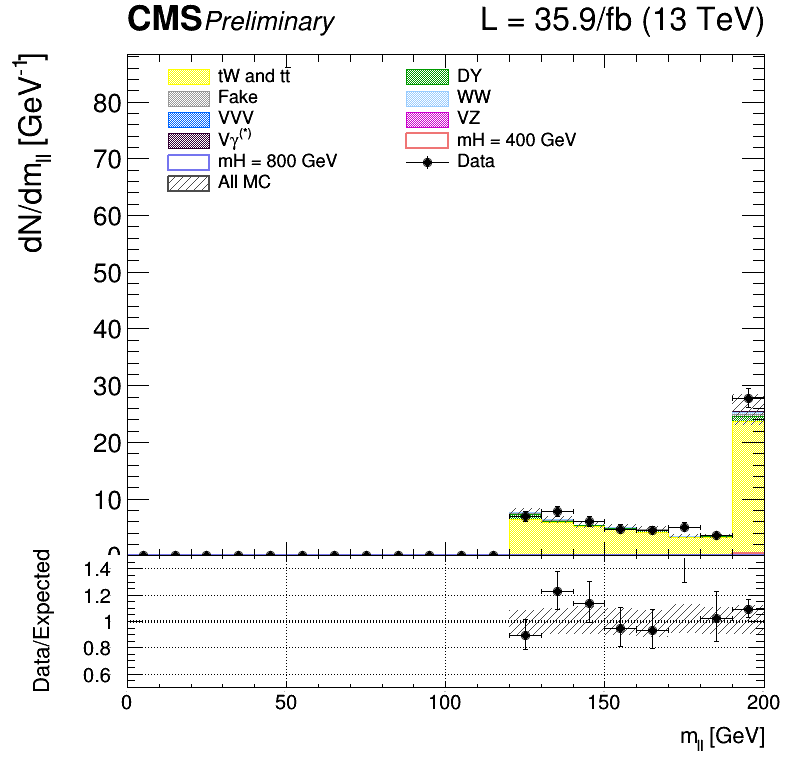
\includegraphics[width=0.45\textwidth]{../AN/Figs/SF_CR_Blind/cratio_hww2l2v_13TeV_top_e_e_2j_VBF_mll_DY.png}
}\\

\subfigure[$p_T$ leading lepton]{                             
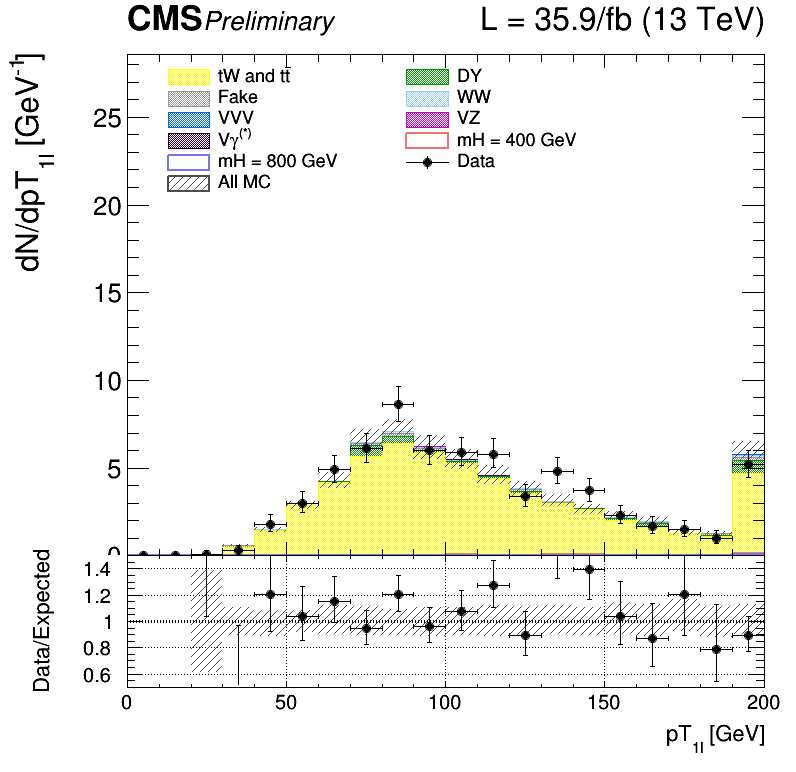
\includegraphics[width=0.45\textwidth]{../AN/Figs/SF_CR_Blind/cratio_hww2l2v_13TeV_top_e_e_2j_VBF_std_vector_lepton_pt[0].png}
}                                              
\subfigure[$p_T^{\ell \ell}$]{                               
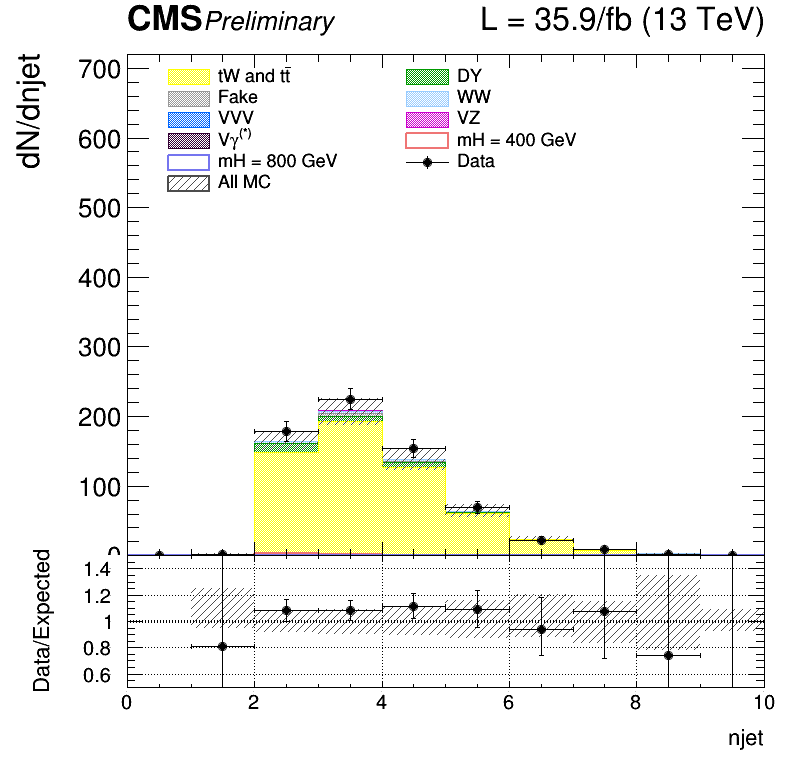
\includegraphics[width=0.45\textwidth]{../AN/Figs/SF_CR_Blind/cratio_hww2l2v_13TeV_top_e_e_2j_VBF_njet.png}
}\\

\caption{Control plots for several variables in a Top enriched phase space for ee.}
    \label{fig:mll_sigSF_CR_top_ee}
\end{figure}




\begin{figure}[htbp]
\centering
\subfigure[$m_T^I$]{
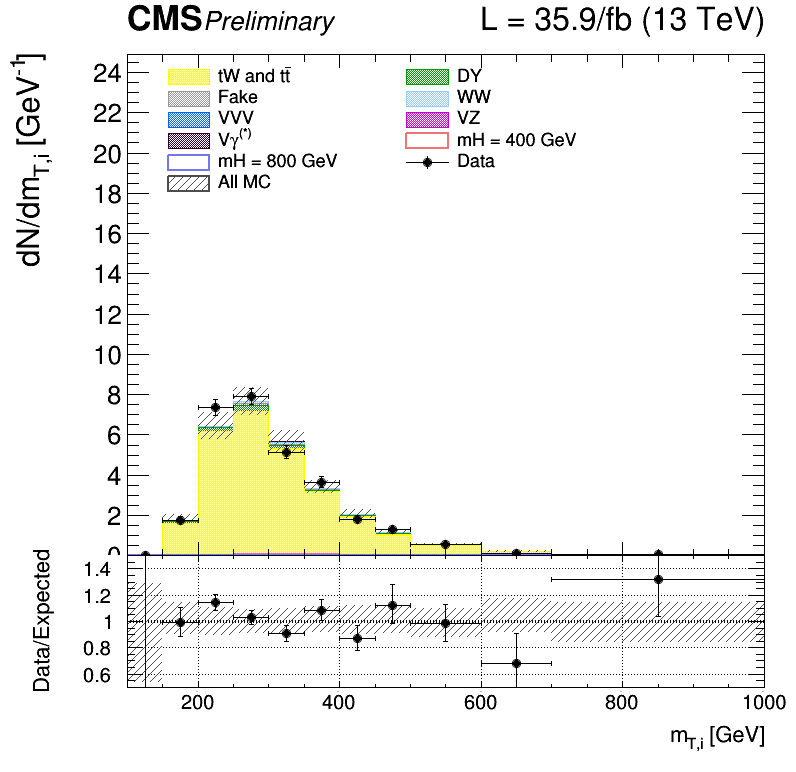
\includegraphics[width=0.45\textwidth]{../AN/Figs/SF_CR_Blind/cratio_hww2l2v_13TeV_top_mu_mu_2j_VBF_mTi.png}
}
\subfigure[$m_T^H$]{
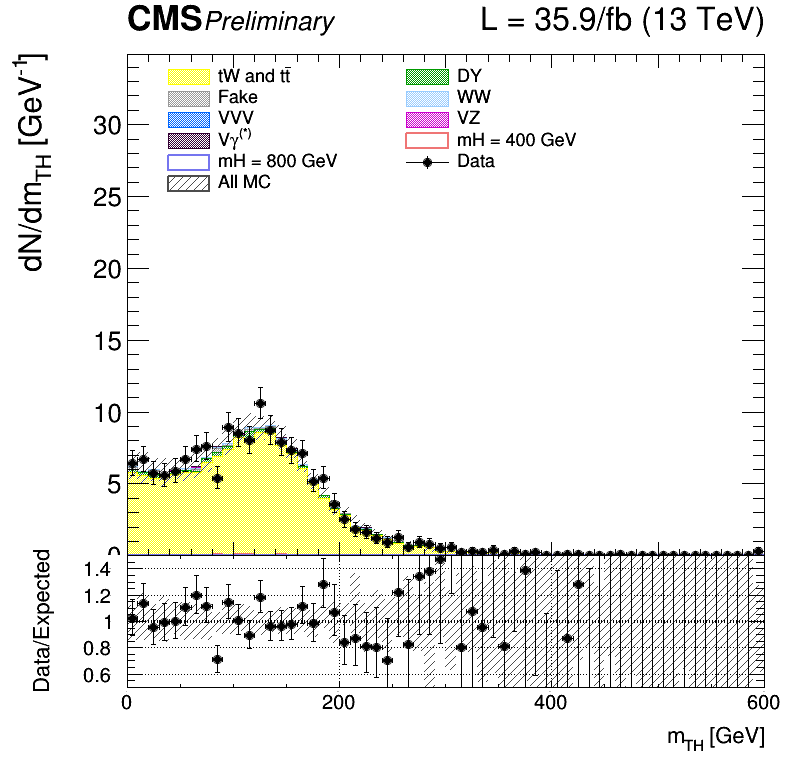
\includegraphics[width=0.45\textwidth]{../AN/Figs/SF_CR_Blind/cratio_hww2l2v_13TeV_top_mu_mu_2j_VBF_mth.png}
}                                              
\\                                             
\subfigure[$m_{jj}$]{                             
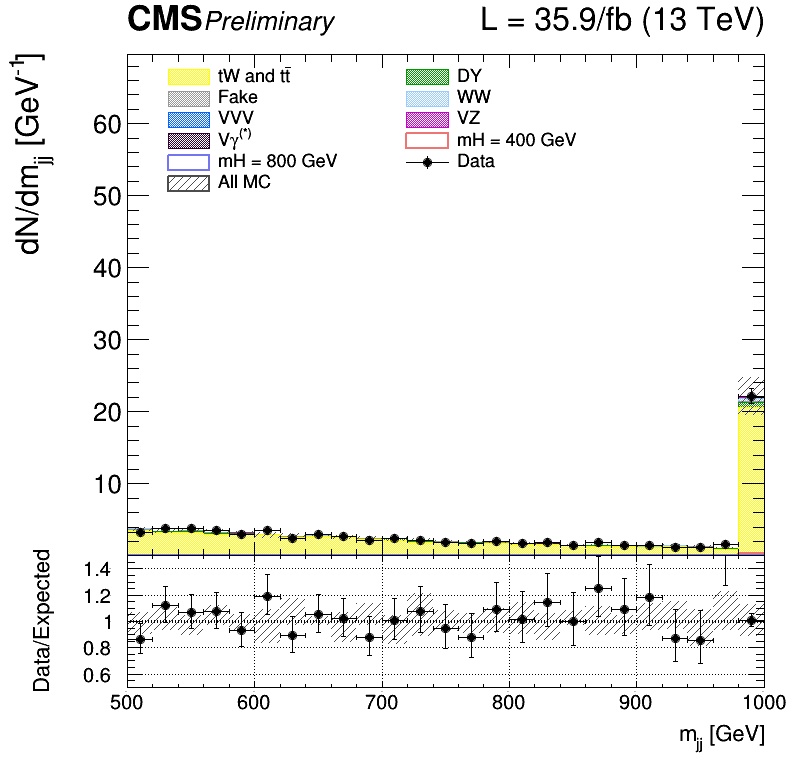
\includegraphics[width=0.45\textwidth]{../AN/Figs/SF_CR_Blind/cratio_hww2l2v_13TeV_top_mu_mu_2j_VBF_mjj_DY.png}
}                                              
\subfigure[$m_{\ell \ell}$]{                               
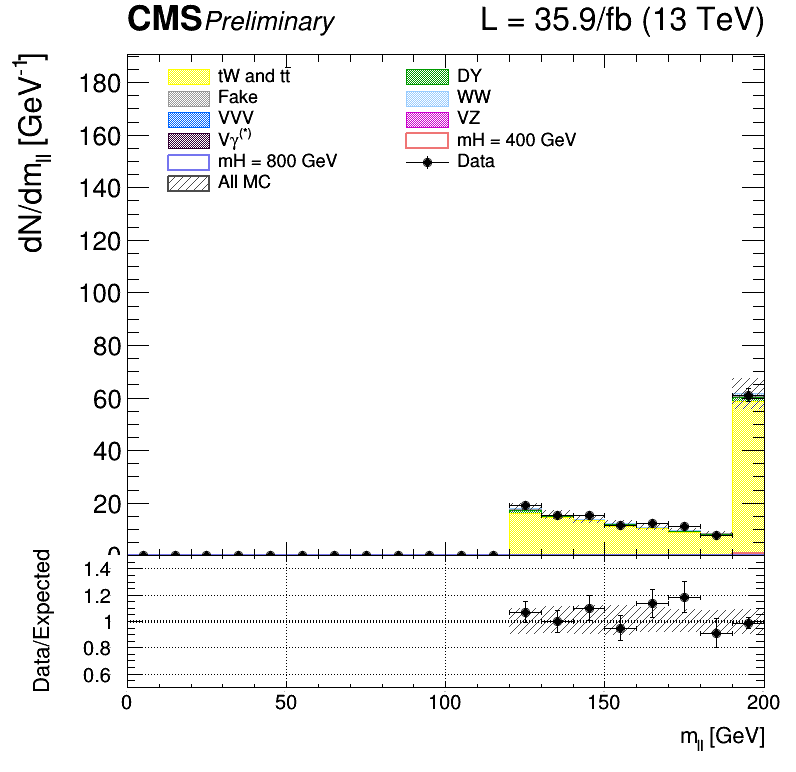
\includegraphics[width=0.45\textwidth]{../AN/Figs/SF_CR_Blind/cratio_hww2l2v_13TeV_top_mu_mu_2j_VBF_mll_DY.png}
}\\

\subfigure[$p_T$ leading lepton]{                             
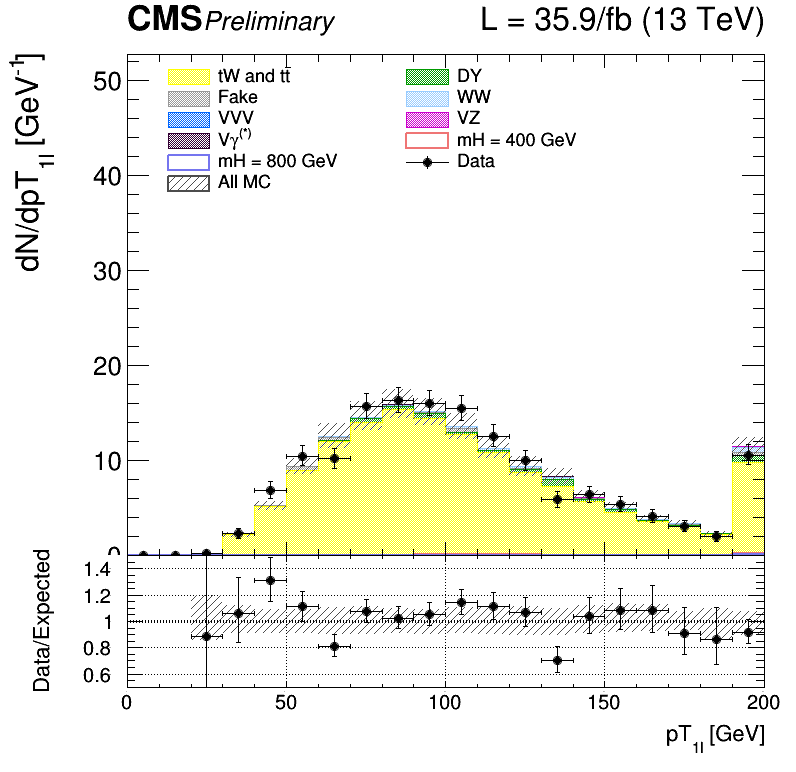
\includegraphics[width=0.45\textwidth]{../AN/Figs/SF_CR_Blind/cratio_hww2l2v_13TeV_top_mu_mu_2j_VBF_std_vector_lepton_pt[0].png}
}                                              
\subfigure[$p_T^{\ell \ell}$]{                               
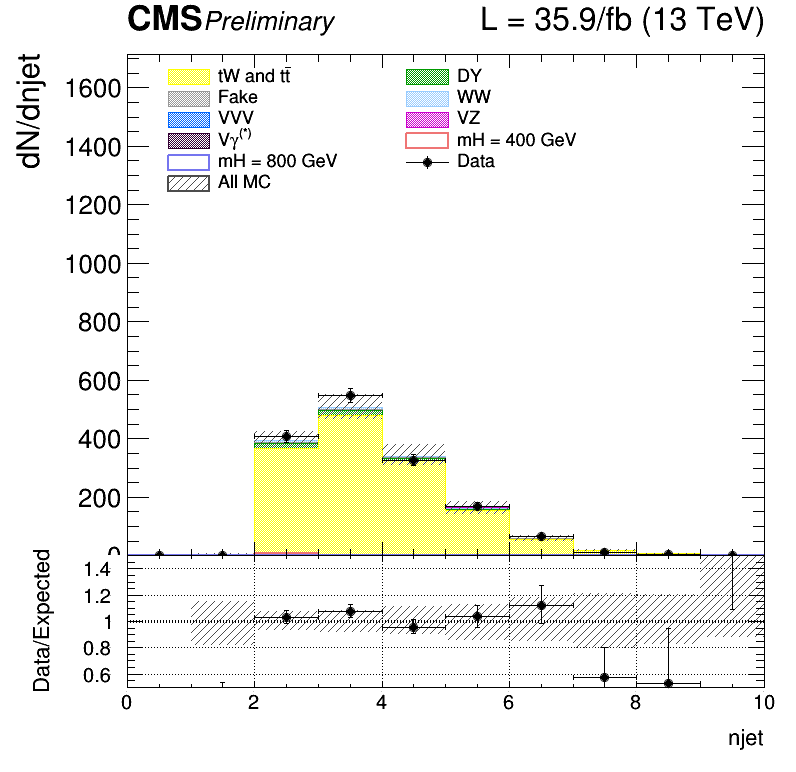
\includegraphics[width=0.45\textwidth]{../AN/Figs/SF_CR_Blind/cratio_hww2l2v_13TeV_top_mu_mu_2j_VBF_njet.png}
}\\

\caption{Control plots for several variables in a Top enriched phase space for $\mu \mu$.}
    \label{fig:mll_sigSF_CR_top_mm}
\end{figure}



